A eletrônica embarcada do projeto tem como base 3 microcontroladores: o Arduino, o Raspberry Pi e o Galileo.

\begin{figure}[H]
	\centering
	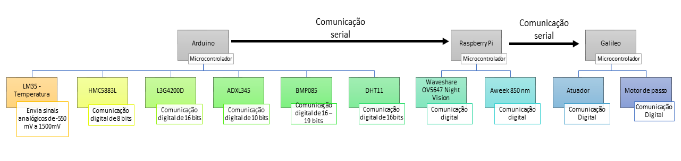
\includegraphics[width=0.8\textwidth]{figuras/eletronicaembarcadasum}
	\caption{Funcionamento geral da eletrônica embarcada no SUM.}
	\label{img:eletronicaembarcadasum}
\end{figure}

A Figura \ref{img:eletronicaembarcadasum} mostra o funcionamento geral da eletrônica embarcada do projeto. Os sensores que auxiliarão na estabilização do balão serão: LM35(Temperatura), HMC5883L(Bússola), L3G4200D(movimento), ADXL345(acelerometro), BMP085(pressão) e DHT11(umidade). Estes sensores estarão conectados em um Arduino UNO que, por sua vez, interpretará os dados dos sensores e mandará suas informações em série para o Raspberry Pi, que também estará conectado a um painel composto por vários LEDs para iluminação em infravermelho, o Aweek. Por fim, O Raspberry Pi mandará as informações para o microcontrolador Intel Galileo Gen 2, indicando se será necessária a estabilização da estrutura, de acordo com a interpretação feita pelo Arduino. Caso seja necessária a estabilização, o Galileo decidirá se ativará um motor de passo para realizar a estabilização através do trilho situado na payload, ou se ativará o atuador Reaction Wheel.

Raspberry Pi estará sendo utilizado também para transmitir as imagens em tempo real para a central. Ele receberá os dados da câmera, através do seu conector específico para câmera, e cada balão passará as informações para o balão mais próximo da central, a comunicação entre eles será sem fio montando uma rede intranet. O balão que esta recebendo tudo, transmitirá para a central através de um cabo de ethernet e o computador que recebe realizará todo o procedimento desejado com as imagens.

\subsection{Microcontroladores e microprocessadores}

Os microcontroladores e microprocessadores serão responsáveis por integrar todas as atividades do sistema, seja a aquisição, armazenamento, transmissão de dados, obtidos por sensores ou câmeras, conversão de dados analógicos em digitais ou o controle do sistema. Essas atividades exigirão determinados requisitos, de acordo com a sua aplicação. Logo, vê-se a necessidade de especificar os microprocessadores e microcontroladores responsáveis por cada setor. A iniciativa de usar um microcontrolador é baseada no fato deste possuir diversos periféricos e um processador embutidos em um único circuito integrado. Esta característica minimiza o tamanho físico do projeto e facilita a implementação de várias aplicações \cite{prado2009implementaccao}.  Contudo, as CPUs dos microcontroladores são menos poderosas do que as dos microprocessadores, suas instruções, geralmente, se limitam às instruções mais simples, sua frequência de clock é menor e seu espaço de memória endereçável costuma ser menor \cite{rucinski}.

Em condições desfavoráveis, como por exemplo um fluxo de ar inesperado, a rápida estabilização do balão se mostra essencial para a captação das imagens, visando sua qualidade. O setor voltado para o controle e estabilização exigirá uma frequência de clock muito alta, pois esta deverá ser realizada rapidamente. Portanto, essa função será desempenhada pelo Intel Galileo Gen 2, pois este admite frequências de clock de até 400 MHz. Além disso, é compatível com os shields feitos para Arduino UNO e com o seu ambiente de desenvolvimento (IDE), o que torna sua codificação mais prática.

Para os setores de armazenamento e transmissão de imagens das câmeras, o Raspberry PI 2 foi considerado o ideal, dado sua eficiência em termos de processamento de dados. Outra vantagem de se utilizar o Raspberry é a sua compatibilidade com a linguagem Python, o que facilitará o desenvolvimento do algoritmo responsável pela compressão de vídeo.

Para o setor voltado para a captação de dados dos sensores, decidiu-se que o ideal seria utilizar o Arduino UNO, visto que este possui grande compatibilidade com os shields escolhidos, além de uma quantidade razoável de portas disponíveis.

As especificações dos microcontroladores estão relacionadas na tabela \ref{table:microprocessadores}:

\begin{table}[H]
\centering
\begin{tabular}{p{3cm}|p{3cm}|p{3cm}|p{3cm}|}
\cline{2-4}
 & Intel Galileo Gen 2 & Raspberry PI 2 & Arduino UNO \\ \hline
\multicolumn{1}{|l|}{Microcontrolador} & \multicolumn{1}{c|}{-} & \multicolumn{1}{c|}{-} & ATmega328 \\ \hline
\multicolumn{1}{|l|}{Processador} & SoC Quark X1000 - 32 bits & Broadcom BCM2836 SoC & \multicolumn{1}{c|}{-} \\ \hline
\multicolumn{1}{|l|}{Arquitetura} & x86 & Quad-core ARM Cortex-A7 & \multicolumn{1}{c|}{-} \\ \hline
\multicolumn{1}{|l|}{Memória} & DDR3 de 256 MB, SRAM embarcada de 512 KB, NOR Flash de 8 MB e EEPROM padrão de 8 KB on-board & 1 GB de RAM & 32K (0.5 usado pelo bootloader) \\ \hline
\multicolumn{1}{|l|}{Clock} & 400 MHz & 900 MHz & 16MHz \\ \hline
\multicolumn{1}{|l|}{GPU} & \multicolumn{1}{c|}{-} & VídeoCore IV & \multicolumn{1}{c|}{-} \\ \hline
\multicolumn{1}{|l|}{Portas analógicas} & 6 & \multicolumn{1}{c|}{-} & 6 \\ \hline
\multicolumn{1}{|l|}{Portas digitais} & 14 & 26 (GPIO) & 14 \\ \hline
\multicolumn{1}{|l|}{Portas PWM} & 6 (12-bit) & \multicolumn{1}{c|}{-} & 6 \\ \hline
\multicolumn{1}{|l|}{Tensão de operação} & 12 V & 5 V & 5 V \\ \hline
\multicolumn{1}{|l|}{Corrente máxima} & 2 A & 1 A & 40 mA \\ \hline
\multicolumn{1}{|l|}{Alimentação} & 7 - 15 V & 5 V & 7 -12 Vdc \\ \hline
\multicolumn{1}{|l|}{Interface Ethernet} & 10/100 Mbps & 10/100 Mbps & \multicolumn{1}{c|}{-} \\ \hline
\multicolumn{1}{|l|}{Saída de vídeo e Áudio} & \multicolumn{1}{c|}{-} & HDMI e Av & \multicolumn{1}{c|}{-} \\ \hline
\end{tabular}
\caption{Fontes: \cite{intelGalileo}, \cite{rsppi}, \cite{arduino}.}
\label{table:microprocessadores}
\end{table}

\subsection{Sensores}

Para os sensores utilizados nesse projeto que já possuem internamente um conversor de sinal analógico para digital e também um filtro para reduzir ruídos, o funcionamento é basicamente coletar a informação desejada, fazer a conversão de dados para digital, logo após realiza a filtragem e realizada a filtragem esses dados são passados para uma memória e para um bloco onde vai controlar essas informações no sistema de comunicação I2C.

O sistema de comunicação I2C possibilita utilizar, em um mesmo sistema, componentes de tecnologias construtivas diferentes sem que haja incompatibilidade e nem conflitos na comunicação.

A transmissão da informação entre os dispositivos é feita através de dois fios, serial data DAS e serial clock SCL.

\begin{figure}[H]
	\centering
	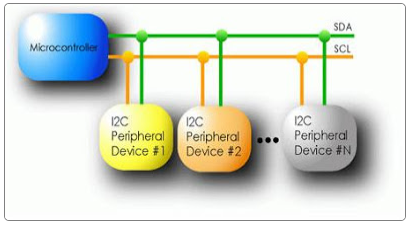
\includegraphics[width=0.8\textwidth]{figuras/1}
	\caption{Exemplo de funcionamento da comunicação I2C \cite{microcontrolandos}.}
	\label{img:funcionamentoI2c}
\end{figure}

Os dispositivos ligados em Inter IC possuem um endereço fixo (cada componente recebe um endereço específico), e podemos configurá-los para receber ou transmitir dados; dessa maneira eles podem ser classificados de várias formas, como: mestres (MASTER), escravos (SLAVE), entre outras.

Uma das vantagens do padrão I2C é que ele não fixa a velocidade de transmissão (freqüência), pois ela será determinada pelo circuito MASTER (transmissão do SCL).

O Diagrama de funcionamento dos sensores são demonstrados nas figuras de \ref{img:acelerometro} à \ref{img:sensorumidade}.

\begin{itemize}
  \item Acelerômetro
  \begin{figure}[H]
    \centering
    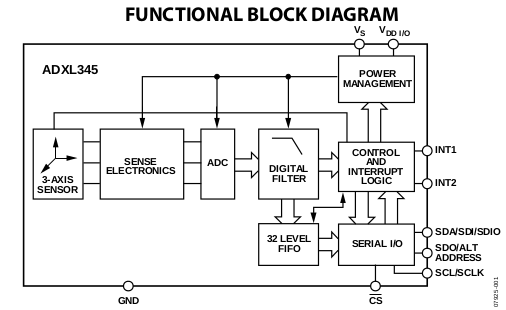
\includegraphics[width=0.8\textwidth]{figuras/2}
    \caption{Diagrama funcional acelerômetro ADXL345 \cite{acelerometro}.}
    \label{img:acelerometro}
  \end{figure}
  \item Barômetro
  \begin{figure}[H]
    \centering
    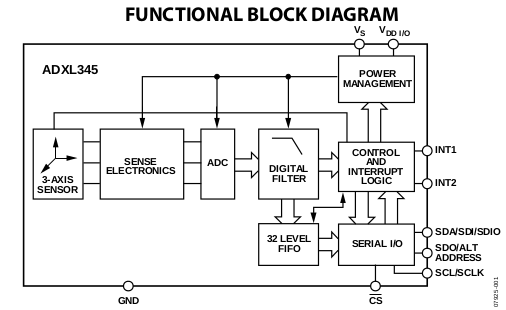
\includegraphics[width=0.8\textwidth]{figuras/2}
    \caption{Diagrama funcional Barômetro BMP085 \cite{barometro}.}
    \label{img:barometro}
  \end{figure}
  \item Giroscópio
  \begin{figure}[H]
    \centering
    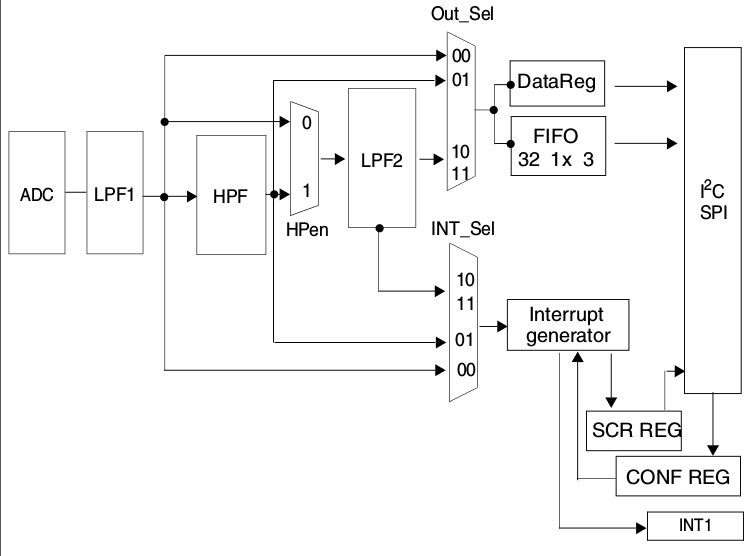
\includegraphics[width=0.8\textwidth]{figuras/4}
    \caption{Diagrama Funcional Giroscópio L3G4200D \cite{giroscopio}.}
    \label{img:giroscopio}
  \end{figure}
  \item Magnetômetro
  \begin{figure}[H]
    \centering
    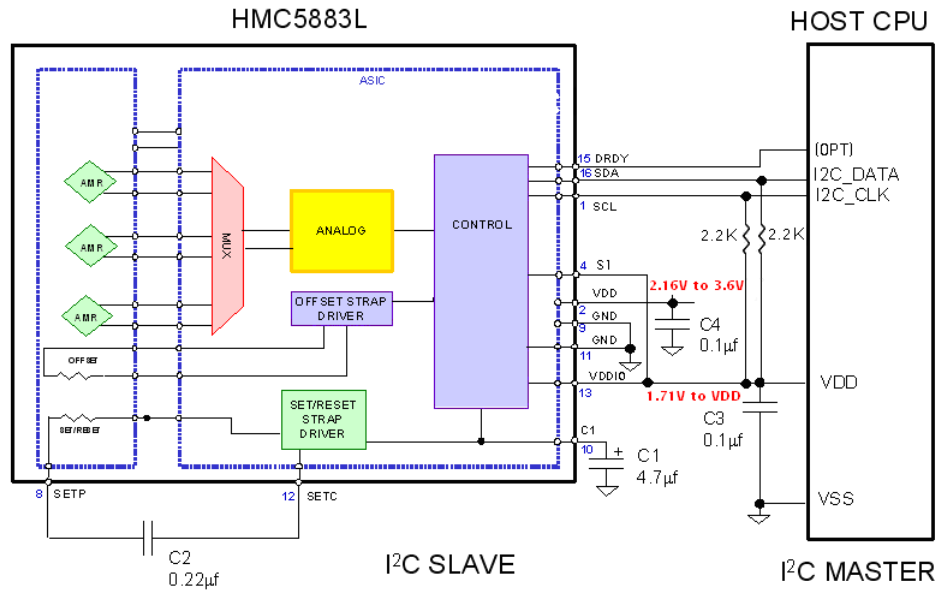
\includegraphics[width=0.8\textwidth]{figuras/6}
    \caption{Diagrama funcional magnetômetro HMC5883L \cite{magnetometro}.}
    \label{img:magnetometro}
  \end{figure}
  \item Sensor de umidade
  \begin{figure}[H]
    \centering
    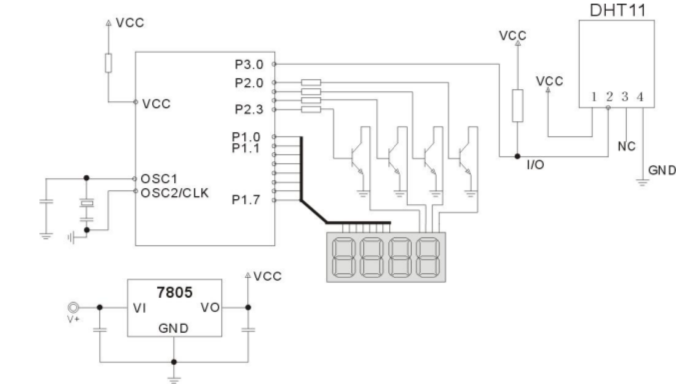
\includegraphics[width=0.8\textwidth]{figuras/5}
    \caption{Diagrama funcional sensor de umidade \cite{sensorhumidade}.}
    \label{img:sensorumidade}
  \end{figure}
\end{itemize}

A conversão Analógico/Digital será feita internamente nos sensores, como foi mostrado em seus respectivos diagramas funcionais, o que significa que fornecerão valores digitais em suas saídas, que estarão conectadas a um microcontrolador.

Geralmente, os microcontroladores processam dados obtidos por sensores e na sua saída são encontrados valores analógicos, logo é necessário transformá-los em valores digitais. Então, para executar essa atividade, é preciso do conversor A/D, que inter-faceiam os dispositivos de medidas e o microcontrolador.

Nesses conversores, quanto maior o número bits de saída, melhor ele será. Por exemplo, um conversor que tem uma saída de quatro bits possui dezesseis degraus de indicação, ou seja, pode definir uma escala de dezesseis valores diferentes.

\begin{figure}[H]
  \centering
  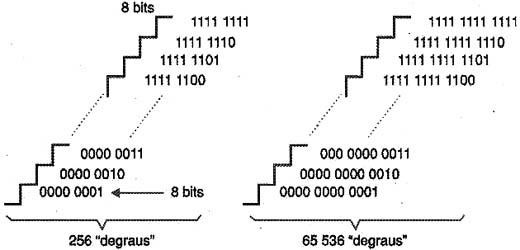
\includegraphics[width=0.8\textwidth]{figuras/ADC}
  \caption{Ilustração da escala de bits.}
  \label{img:escaladebits}
\end{figure}

Se o circuito converte sinais na faixa de 0V a 1V, é preciso ter cuidado para que os sensores usados trabalhem nessa faixa. Um amplificador operacional pode ter um ganho programado para evitar esses problemas. Então, as saídas terão um número n de pinos nas quais as saídas nos níveis lógicos 0 ou 1 são obtidos conforme a tensão de entrada \cite{conversoresad}.
